\paperchapter{November 2023}{26 November 2023}{A}{50}{17th GSET}
\keytable{\kcell{1}{A} & \kcell{2}{A} & \kcell{3}{A} & \kcell{4}{B} & \kcell{5}{B} & \kcell{6}{B} & \kcell{7}{B} & \kcell{8}{C} & \kcell{9}{A} & \kcell{10}{C} \\
\kcell{11}{A} & \kcell{12}{D} & \kcell{13}{B} & \kcell{14}{B} & \kcell{15}{A} & \kcell{16}{C} & \kcell{17}{D} & \kcell{18}{B} & \kcell{19}{C} & \kcell{20}{A} \\
\kcell{21}{A} & \kcell{22}{B} & \kcell{23}{A} & \kcell{24}{D} & \kcell{25}{C} & \kcell{26}{A} & \kcell{27}{B} & \kcell{28}{A} & \kcell{29}{C} & \kcell{30}{A} \\
\kcell{31}{C} & \kcell{32}{C} & \kcell{33}{C} & \kcell{34}{C} & \kcell{35}{B} & \kcell{36}{B} & \kcell{37}{B} & \kcell{38}{D} & \kcell{39}{C} & \kcell{40}{Z} \\
\kcell{41}{A} & \kcell{42}{A} & \kcell{43}{D} & \kcell{44}{B} & \kcell{45}{C} & \kcell{46}{C} & \kcell{47}{B} & \kcell{48}{A} & \kcell{49}{C} & \kcell{50}{A}}
\begin{question}{1}
{Match X with Y.\\[2pt]
\begin{tabular}{@{}ll@{}}
\textbf{X} & \textbf{Y}\\
1. Proxemics & a. Use of touch\\
2. Kinesics & b. Use of body language\\
3. Haptics & c. Use of space\\
\end{tabular}\par}
\optsfour{1-c, 2-b, 3-a}{1-a, 2-b, 3-c}{1-b, 2-a, 3-c}{1-c, 2-a, 3-b}
\answer{A}{1-c, 2-b, 3-a}
\begin{explain}
\textbf{Proxemics} is the use of \emph{space} (c), \textbf{Kinesics} the use of \emph{body language} such as gestures, posture and facial expression (b), and \textbf{Haptics} the use of \emph{touch} (a). The match is 1-c, 2-b, 3-a.
\tip{Non-verbal codes: Kinesics (body), Proxemics (space), Haptics (touch), Chronemics (time), Paralanguage (voice qualities), Oculesics (eye contact), Artifacts (dress and objects).}
\end{explain}
\end{question}

\begin{question}{2}
{Use of 'space' in communication is called\par}
\optsfour{Proximics}{Chronomics}{Para language}{Haptics}
\answer{A}{Proximics}
\begin{explain}
The use of space and distance in communication is \textbf{Proxemics} (Edward T.~Hall). Hall described four zones: intimate (0--18 in), personal (1.5--4 ft), social (4--12 ft) and public (over 12 ft).
\why{Chronemics = use of time; Paralanguage = tone, pitch, pace and other vocal cues; Haptics = touch.}
\end{explain}
\end{question}

\begin{question}{3}
{The connotative meaning of a word is\par}
\optstwo{Subjective meaning}{Oppositive meaning}{Donotative meaning}{Real meaning}
\answer{A}{Subjective meaning}
\begin{explain}
\textbf{Connotative meaning} is the associated, emotional or \emph{subjective} meaning that a word carries beyond its dictionary sense. For example, ``home'' connotes warmth and security. \textbf{Denotative} meaning is the literal, dictionary (``real'') meaning.
\end{explain}
\end{question}

\begin{question}{4}
{In the process of communication, the receiver\par}
\optstwo{Encodes the message}{Decodes the message}{Is a channel}{Has no role}
\answer{B}{Decodes the message}
\begin{explain}
The receiver \textbf{decodes} the message, interpreting the symbols to extract meaning. The sender encodes, and the channel carries the message.
\end{explain}
\end{question}

\begin{question}{5}
{'Demophobia' refers to\par}
\optstwo{Fear of death}{Fear of crowd}{Fear of speaking}{Fear of failure}
\answer{B}{Fear of crowd}
\begin{explain}
\textbf{Demophobia} (Greek \emph{demos}, people) is the fear of crowds. It is also called enochlophobia or ochlophobia.
\why{Fear of death = thanatophobia; fear of public speaking = glossophobia; fear of failure = atychiphobia.}
\end{explain}
\end{question}

\begin{question}{6}
{Which of the following institutions responsible for quality technical and Management Higher Education in India?\par}
\optsfour{NCERT}{AICTE}{NCTE}{NIEPA}
\answer{B}{AICTE}
\begin{explain}
The \textbf{All India Council for Technical Education (AICTE)}, a statutory body under the AICTE Act 1987 (set up as an advisory body in 1945), regulates and ensures the quality of \emph{technical and management} education: engineering, pharmacy, architecture, MBA/PGDM and MCA.
\why{NCERT deals with school curriculum; NCTE with teacher education; NIEPA with educational planning and administration.}
\end{explain}
\end{question}

\begin{question}{7}
{'NAAC' assessment cycle is for\par}
\optsfour{3 years}{5 years}{10 years}{7 years}
\answer{B}{5 years}
\begin{explain}
NAAC accreditation is valid for \textbf{5 years}, after which an institution must undergo the next cycle of assessment and accreditation. (NAAC was established in 1994 by UGC and is headquartered in Bengaluru.)
\end{explain}
\end{question}

\begin{question}{8}
{The National Education Day in India is celebrated every year on\par}
\optsfour{14th November}{5th September}{11th November}{2nd October}
\answer{C}{11th November}
\begin{explain}
\textbf{National Education Day} is observed on \textbf{11 November}, the birth anniversary of \emph{Maulana Abul Kalam Azad}, India's first Education Minister (1947--58). It has been celebrated since 2008.
\why{14 November is Children's Day (Nehru), 5 September is Teachers' Day (Dr.~S.~Radhakrishnan), and 2 October is Gandhi Jayanti.}
\end{explain}
\end{question}

\begin{question}{9}
{What is the full form of ABC, according to NEP (2020) ?\par}
\optstwo{Academic Bank of Credits}{Academic Bank of Certification}{Annual Book of Credits}{Academic Basic Certification}
\answer{A}{Academic Bank of Credits}
\begin{explain}
NEP~2020 proposed an \textbf{Academic Bank of Credits (ABC)}, a digital store of the credits earned by students from recognised HEIs. It enables multiple entry and exit, credit transfer and lifelong learning. The UGC ABC Regulations were notified in 2021.
\end{explain}
\end{question}

\begin{question}{10}
{According to NIRF overall ranking 2023, which institution ranked one in India?\par}
\optstwo{IISc, Bangalore}{IISER, Pune}{IIT, Madras}{IIM, Ahmedabad}
\answer{C}{IIT, Madras}
\begin{explain}
In \textbf{NIRF 2023} (Overall category), \textbf{IIT Madras} was ranked first, as it has been every year since 2019. IISc Bengaluru was 2nd and IIT Delhi 3rd. (IISc tops the \emph{University} category.)
\end{explain}
\end{question}

\begin{question}{11}
{Which of the following diagrams correctly represents the relationship among tennis fans, cricket players and students?\par}
\optsfour{\tikz[baseline=-0.5ex,scale=0.28]{\draw (0,0.45) circle(1); \draw (-0.55,-0.45) circle(1); \draw (0.55,-0.45) circle(1);}}{\tikz[baseline=-0.5ex,scale=0.28]{\draw (0,0) circle(1); \draw (1.4,0) circle(1); \draw (2.8,0) circle(1);}}{\tikz[baseline=-0.5ex,scale=0.28]{\draw (0,0) circle(1.2); \draw (0,0) circle(0.8); \draw (0,0) circle(0.4);}}{\tikz[baseline=-0.5ex,scale=0.28]{\draw (0,0) circle(1.2); \draw (0,0) circle(0.6); \draw (2.2,0) circle(0.7);}}
\answer{A}{\tikz[baseline=-0.5ex,scale=0.28]{\draw (0,0.45) circle(1); \draw (-0.55,-0.45) circle(1); \draw (0.55,-0.45) circle(1);}}
\begin{explain}
None of the three groups is contained in another, and any two (or all three) can share members. A student may be a tennis fan, a cricket player may be a student, and a student who plays cricket may also be a tennis fan. So the diagram must show \textbf{three mutually overlapping circles} with a common central region, which is option (A).
\begin{center}
\begin{tikzpicture}[scale=0.75,font=\scriptsize]
\draw[fill=brand!10,fill opacity=0.5] (0,0.55) circle(1); \node at (0,1.8) {Tennis fans};
\draw (-0.65,-0.5) circle(1); \node[left] at (-1.65,-0.6) {Cricket players};
\draw (0.65,-0.5) circle(1); \node[right] at (1.65,-0.6) {Students};
\end{tikzpicture}
\end{center}
\end{explain}
\end{question}

\begin{question}{12}
{'Umpire' is related to 'Match' in the same way as 'Judge' is related to\par}
\optsfour{Court}{Lawyer}{Judgement}{Law suit}
\answer{D}{Law suit}
\begin{explain}
An \textbf{umpire} presides over and gives decisions in a \textbf{match}; likewise, a \textbf{judge} presides over and decides a \textbf{law suit} (case). The relation is \emph{adjudicator : the event being adjudicated}.
\why{A court is the \emph{place} (the analogue of the stadium), a lawyer is a participant, and a judgement is the decision itself (the analogue of the umpire's ruling).}
\end{explain}
\end{question}

\begin{question}{13}
{In question below is given a statement followed by assumptions numbered I and II. Consider the statement and decide which of the given assumption is implicit ?\newline Statement: If you want to give any advertisement give it in newspaper "X" - A tells to B.\newline Assumptions: \newline I. 'B' wants to publicise his products.\newline II. Newspaper 'X' has a wide circulation.\par}
\optstwo{Only assumption I is implicit}{Only assumption II is implicit}{Either I or II is implicit}{Neither I nor II is implicit}
\answer{B}{Only assumption II is implicit}
\begin{explain}
A advises B to advertise in newspaper X. This advice assumes that X reaches many people, i.e.\ that it has a wide circulation, so assumption II is implicit. The statement is conditional (``\emph{If} you want to give any advertisement \ldots''), so it does not assume that B actually wants to publicise products. Assumption I is not implicit.
\textbf{Only II is implicit.}
\end{explain}
\end{question}

\begin{question}{14}
{P, Q, R, S and U are the family members. P and Q are real brothers. R is a sister of P. S is a father of P. U is a father of S. What is the relation between P and U?\par}
\optstwo{Granddaughter and grandfather}{Grandson and grandfather}{Father and son}{Father and daughter}
\answer{B}{Grandson and grandfather}
\begin{explain}
S is P's father and U is S's father, so U is P's paternal \textbf{grandfather}. P is a ``real brother'' of Q, so P is male, a \textbf{grandson}.
\begin{center}
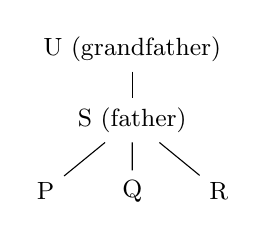
\begin{tikzpicture}[font=\small,level distance=9mm,sibling distance=11mm]
\node{U (grandfather)} child{node{S (father)} child{node{P}} child{node{Q}} child{node{R}}};
\end{tikzpicture}
\end{center}
\end{explain}
\end{question}

\begin{question}{15}
{Find the next term of given series.\newline A7T, E12Q, I19L, \blank{}\par}
\optsfour{M28E}{M25E}{M24C}{M29E}
\answer{A}{M28E}
\begin{explain}
Three independent patterns:
\begin{itemize}
\item First letters: A, E, I, \textbf{M} (+4 each).
\item Numbers: 7, 12, 19, \textbf{28} (+5, +7, +9).
\item Last letters: T, Q, L, \textbf{E} ($-3$, $-5$, $-7$: T(20)$\rightarrow$Q(17)$\rightarrow$L(12)$\rightarrow$E(5)).
\end{itemize}
The next term is \textbf{M28E}.
\end{explain}
\end{question}

\begin{question}{16}
{Which of the following are a web browser?\newline 1. Microsoft edge\newline 2. Google chrome\newline 3. Mozilla firefox\newline 4. Opera\newline 5. Safari\par}
\optstwo{1, 2, 3 and 4}{1, 2, 4 and 5}{1, 2, 3, 4 and 5}{1, 2, 3 and 5}
\answer{C}{1, 2, 3, 4 and 5}
\begin{explain}
All five are web browsers: Microsoft Edge, Google Chrome, Mozilla Firefox, Opera and Apple Safari. The answer is 1, 2, 3, 4 and 5.
\end{explain}
\end{question}

\begin{question}{17}
{Which of the following are used in video-conferencing ?\newline 1. Google Meet\newline 2. Microsoft Team\newline 3. Cisco WebEx\newline 4. Skype\newline 5. Zoom meeting\par}
\optstwo{1, 2, 3 and 5}{1, 2, 4 and 5}{1, 3, 4 and 5}{1, 2, 3, 4 and 5}
\answer{D}{1, 2, 3, 4 and 5}
\begin{explain}
All five are video-conferencing tools: Google Meet, Microsoft Teams, Cisco WebEx, Skype and Zoom. The answer is (D).
\end{explain}
\end{question}

\begin{question}{18}
{The first page of website is called\par}
\optsfour{Main page}{Home page}{Front page}{Open page}
\answer{B}{Home page}
\begin{explain}
The first (main entry) page of a website is its \textbf{home page}, usually reached at the site's root URL (e.g.\ \texttt{www.example.com/}). It links to all other sections of the site.
\end{explain}
\end{question}

\begin{question}{19}
{Given below are two statements:\newline Statement I: SWAYAM stands for study webs of active learning for young aspiring minds.\newline Statement II: All MOOCs on the SWAYAM portal are credit-based MOOCs.\newline In light of the above statements, choose the correct answer from the options given below:\par}
\optsone{Both Statement I and Statement II are true}{Both Statement I and Statement II are false}{Statement I is true but Statement II is false}{Statement I is false but Statement II is true}
\answer{C}{Statement I is true but Statement II is false}
\begin{explain}
\textbf{Statement I} is true: SWAYAM stands for \emph{Study Webs of Active-Learning for Young Aspiring Minds}.
\textbf{Statement II} is false: not all SWAYAM courses are credit-based. Many are non-credit or certificate courses. Credit transfer (up to 40\% of a programme's credits under the UGC SWAYAM Regulations, 2021) applies only to courses so designated and accepted by the parent university.
\end{explain}
\end{question}

\begin{question}{20}
{Given below are two statements, one is labeled as Assertion A and the other is labeled as Reason R.\newline Assertion (A): 'Router' is considered as both input and output device.\newline Reason (R): 'Router' can send data and receive data at the same time.\newline In light of the above statements, choose the correct answer from the options given below:\par}
\optsone{Both (A) and (R) are true and (R) is the correct explanation of (A)}{Both (A) and (R) are true but (R) is not the correct explanation of (A)}{(A) is true but (R) is false}{(A) is false but (R) is true}
\answer{A}{Both (A) and (R) are true and (R) is the correct explanation of (A)}
\begin{explain}
The official key accepts both statements, with R explaining A. A router both \emph{receives} data packets (from a network or modem) and \emph{sends} (forwards) them to other devices, so it performs input and output functions at the same time. Its two-way data transfer is the reason it is treated as both an input and an output device.
\tip{Strictly, a router is a \emph{networking} device. In exam questions, devices that both send and receive data (modem, router, touch screen) are usually accepted as ``input--output'' devices.}
\end{explain}
\end{question}

\begin{question}{21}
{Teaching at higher education should avoid the approach of\par}
\optsone{Covering every bit of content step by step in the class}{Guided learning and self learning}{Motivating learner, use of self learning and lectures on difficult content}{Combination of self learning with digital platform based teaching}
\answer{A}{Covering every bit of content step by step in the class}
\begin{explain}
Higher education aims at developing independent, critical and self-directed learners. \textbf{Covering every bit of content step by step in class} (spoon-feeding) should be avoided. Guided learning, self-learning, motivation, lectures on difficult content and blended digital learning are all desirable.
\end{explain}
\end{question}

\begin{question}{22}
{In Discussion method of teaching which type of questions have limited role ?\par}
\optstwo{Higher order questions}{Yes-no type of questions}{Hypothetical issue related questions}{Critical awareness related questions}
\answer{B}{Yes-no type of questions}
\begin{explain}
A discussion thrives on open-ended, thought-provoking questions. \textbf{Yes/no (closed) questions} have a limited role because they end the exchange with a one-word answer and do not stimulate reasoning or debate.
\end{explain}
\end{question}

\begin{question}{23}
{Which of the following set belongs to teaching?\par}
\optsone{Instruction, scientific inquiry, case study, brainstorming}{Preaching, case study, brainstorming and indoctrination}{Brainstorming, preaching, surmons, instruction}{Tutorial, case study, brainstorming, indoctrination}
\answer{A}{Instruction, scientific inquiry, case study, brainstorming}
\begin{explain}
\textbf{Teaching} involves rational, democratic activities that respect the learner's reasoning: instruction, scientific inquiry, case study and brainstorming. \textbf{Indoctrination} and \textbf{preaching} (sermons) try to implant beliefs without inviting reasoning, so they are not teaching in the true sense.
\why{Options (B), (C) and (D) each contain preaching, sermons or indoctrination.}
\end{explain}
\end{question}

\begin{question}{24}
{Which of the following set of variables of learner largely influence the learning outcomes?\par}
\optsone{Motivation, comprehension, gender, cognition}{Study habit, religion, motivation, socio-economic status}{Religion, socio-economic status, vocabulary, cognition}{Cognition, study habit, comprehension, motivation}
\answer{D}{Cognition, study habit, comprehension, motivation}
\begin{explain}
The learner variables that largely determine learning outcomes are psychological and academic: \textbf{cognition} (intellectual ability), \textbf{study habits}, \textbf{comprehension} and \textbf{motivation}.
\why{Gender and religion are not determinants of learning outcomes, so any set containing them is wrong.}
\end{explain}
\end{question}

\begin{question}{25}
{Characteristics of teaching as profession does not ensure\par}
\optsone{Having a code of conduct}{Freedom to work independently}{Good earning and family life}{Freedom of research and student counselling}
\answer{C}{Good earning and family life}
\begin{explain}
Teaching as a profession is characterised by a \textbf{code of conduct (ethics)}, \textbf{professional autonomy} (freedom to work independently) and \textbf{academic freedom} in research and counselling. A \textbf{good income and family life} is a personal benefit, not a defining characteristic that the profession ensures.
\end{explain}
\end{question}

\begin{question}{26}
{Which of the following are Sustainable Development Goals (SDGs)?\newline 1. Clean water and sanitation\newline 2. Deforestation\newline 3. Climate action\newline 4. Quality education\newline 5. Affordable and clean energy\newline Choose the correct answer from the options given below :\par}
\optsfour{1, 3, 4 and 5}{1, 3 and 5}{1, 2, 3 and 5}{1, 3 and 4}
\answer{A}{1, 3, 4 and 5}
\begin{explain}
SDG~6 (Clean water \& sanitation), SDG~13 (Climate action), SDG~4 (Quality education) and SDG~7 (Affordable \& clean energy) are all goals. \textbf{Deforestation} is a \emph{problem}, not a goal (forests fall under SDG~15, \emph{Life on land}). The answer is 1, 3, 4 and 5.
\end{explain}
\end{question}

\begin{question}{27}
{Match the following and choose the correct option given below:\\[2pt]
\begin{tabular}{@{}ll@{}}
\textbf{G20 Presidency year} & \textbf{Nation}\\
I. 2022 & a. Brazil\\
II. 2023 & b. India\\
III. 2024 & c. South Africa\\
IV. 2025 & d. Indonesia\\
\end{tabular}\par}
\optstwo{I-d, II-b, III-c, IV-a}{I-d, II-b, III-a, IV-c}{I-a, II-b, III-c, IV-d}{I-b, II-c, III-d, IV-a}
\answer{B}{I-d, II-b, III-a, IV-c}
\begin{explain}
G20 presidencies: \textbf{2022 Indonesia} (Bali Summit), \textbf{2023 India} (New Delhi Summit; theme \emph{Vasudhaiva Kutumbakam: One Earth, One Family, One Future}), \textbf{2024 Brazil} (Rio de Janeiro), \textbf{2025 South Africa} (Johannesburg). The match is I-d, II-b, III-a, IV-c.
\end{explain}
\end{question}

\begin{question}{28}
{Recently in February 2023, a large lithium mineral reserve was found in which State ?\par}
\optstwo{Jammu and Kashmir}{Gujarat}{Jharkhand}{Bihar}
\answer{A}{Jammu and Kashmir}
\begin{explain}
In February 2023 the Geological Survey of India announced inferred lithium resources of about \textbf{5.9 million tonnes} in the \textbf{Salal-Haimana area of Reasi district, Jammu \& Kashmir}, India's first major lithium find. Lithium is vital for EV batteries.
\end{explain}
\end{question}

\begin{question}{29}
{Which of the following cyclone has affected the east coast of India in last few years?\newline 1. Cyclone Biparjoy\newline 2. Cyclone Fani\newline 3. Cyclone Taukte\newline 4. Cyclone Amphan\newline Choose the correct answer from the options given below :\par}
\optsfour{1, 2 and 3}{1 and 3}{2 and 4}{1, 3 and 4}
\answer{C}{2 and 4}
\begin{explain}
East-coast (Bay of Bengal) cyclones: \textbf{Fani} (May 2019, Odisha) and \textbf{Amphan} (May 2020, West Bengal).
Biparjoy (2023) and Tauktae (2021) struck the \emph{west} coast (Gujarat). The answer is 2 and 4.
\end{explain}
\end{question}

\begin{question}{30}
{Given below are two statements, one is labeled as Assertion (A) and the other is labeled as Reason (R).\newline Assertion (A): Air Quality Index (AQI) of City-X is 257, while that of City-Y is 65 in the month of August - 2023.\newline Reason (R): City-X is more air polluted than City-Y.\newline In light of the above statements, choose the correct answer from the options given below:\par}
\optsone{Both (A) and (R) are true and (R) is the correct explanation of (A)}{Both (A) and (R) are true but (R) is not the correct explanation of (A)}{(A) is true but (R) is false}{(A) is false but (R) is true}
\answer{A}{Both (A) and (R) are true and (R) is the correct explanation of (A)}
\begin{explain}
An AQI of 257 falls in the \emph{Poor} band (201--300), while an AQI of 65 is \emph{Satisfactory} (51--100). A higher AQI means more air pollution, so City-X is more polluted, and this is exactly what explains the AQI values. Both are true and R explains A.
\end{explain}
\end{question}

\begin{question}{31}
{Scientific method of research involves the process of\par}
\optstwo{Induction}{Deduction}{Indo-deductive method}{Contemplation}
\answer{C}{Indo-deductive method}
\begin{explain}
The scientific method combines \textbf{induction} (observations $\rightarrow$ generalisation or hypothesis) and \textbf{deduction} (hypothesis $\rightarrow$ testable predictions $\rightarrow$ verification). This cycle is called the \textbf{inductive--deductive} method (the ``indo-deductive'' of the option). It is associated with Charles Darwin and John Dewey's reflective thinking.
\end{explain}
\end{question}

\begin{question}{32}
{Snowball sampling method\par}
\optsone{Is most preferred technique during survey method}{Provides representative sample for experimental study}{Is suitable to identify sample from unknown population}{Use rolling ball machine to get random sample}
\answer{C}{Is suitable to identify sample from unknown population}
\begin{explain}
In \textbf{snowball sampling} each respondent refers further respondents, so the sample ``snowballs''. It suits \textbf{hidden, rare or unknown populations} (drug users, migrant workers, rare-disease patients) for which no sampling frame exists.
\why{It is non-probability, so it does not give a representative sample, and it has nothing to do with a rolling-ball machine.}
\end{explain}
\end{question}

\begin{question}{33}
{Which of the following is the correct statement of historical research?\par}
\optsone{It is not a scientific inquiry}{The extrinsic data validation is assumptive}{The findings are subjective to a great extent}{Reveals past with no contribution to future}
\answer{C}{The findings are subjective to a great extent}
\begin{explain}
Historical research reconstructs the past from documents and relics, and the researcher's interpretation plays a large role. Its findings are therefore \textbf{subjective to a great extent}.
\why{It \emph{is} a scientific inquiry. Sources are validated through external criticism (authenticity) and internal criticism (credibility), so validation is not ``assumptive''. It helps us understand the present and plan for the future.}
\end{explain}
\end{question}

\begin{question}{34}
{Which of the following is a discrete variable?\par}
\optstwo{Human IQ score}{Human height}{Number of human beings}{Human weight}
\answer{C}{Number of human beings}
\begin{explain}
A \textbf{discrete variable} takes only separate, countable values (0, 1, 2, \ldots). The \textbf{number of human beings} is counted in whole numbers, so it is discrete.
\why{Height and weight are continuous (they can take any value in a range). IQ is treated as a continuous measure on an interval scale.}
\end{explain}
\end{question}

\begin{question}{35}
{Which of the following statement is true for Swayamprabha ?\par}
\optsone{They are MOOCs and certified for credit consideration by universities}{They are educational programmes under direct-to-home}{One has to pay to subscribe the programme}{They are focussed to the course content from 1st standard to 12th standard}
\answer{B}{They are educational programmes under direct-to-home}
\begin{explain}
SWAYAM Prabha is a group of 40 \textbf{DTH (Direct-to-Home)} educational TV channels telecasting 24$\times$7 via the GSAT-15 satellite. They are \textbf{free}, cover school, higher and lifelong education, and are not credit-bearing MOOCs.
\end{explain}
\end{question}

\begin{question}{36}
{Ravi travelled 4 km straight towards South. He turned left and travelled 6 km straight, then turned right and travelled 4 km straight. How far is he from the starting point ?\par}
\optsfour{8 km}{10 km}{12 km}{15 km}
\answer{B}{10 km}
\begin{explain}
\begin{center}
\begin{tikzpicture}[scale=0.35,font=\scriptsize,>=Stealth]
\draw[thick,->] (0,0) -- node[left]{4} (0,-4);
\draw[thick,->] (0,-4) -- node[above]{6} (6,-4);
\draw[thick,->] (6,-4) -- node[right]{4} (6,-8);
\draw[dashed,accent,thick] (0,0) -- node[below left]{10} (6,-8);
\fill (0,0) circle(4pt) node[left]{Start};
\end{tikzpicture}
\end{center}
South 4 km, left (east) 6 km, right (south) 4 km. Net: 8 km south and 6 km east.
\[\text{Distance}=\sqrt{8^2+6^2}=\sqrt{100}=\mathbf{10\ km}\]
\end{explain}
\end{question}

\begin{question}{37}
{The following diagram shows the number of students who got distinction in the subject out of 500 students.\par}
\qfigure{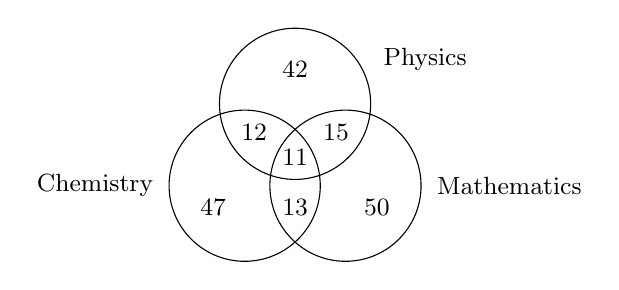
\begin{tikzpicture}[scale=0.8,font=\small]
\draw (0,0.9) circle(1.2); \draw (-0.8,-0.4) circle(1.2); \draw (0.8,-0.4) circle(1.2);
\node at (0,1.45) {42}; \node at (-1.3,-0.75) {47}; \node at (1.3,-0.75) {50};
\node at (-0.65,0.45) {12}; \node at (0.65,0.45) {15}; \node at (0,-0.75) {13}; \node at (0,0.05) {11};
\node[right] at (1.25,1.6) {Physics}; \node[left] at (-2.1,-0.4) {Chemistry}; \node[right] at (2.1,-0.4) {Mathematics};
\end{tikzpicture}}
What is the percentage of students who got distinction only in two subjects?
\optsfour{6\%}{8\%}{10\%}{12\%}
\answer{B}{8\%}
\begin{explain}
``Only two subjects'' means the pairwise overlaps, excluding the centre (11):
\[12\ (\text{P}\cap\text{C})+15\ (\text{P}\cap\text{M})+13\ (\text{C}\cap\text{M})=40\qquad\frac{40}{500}\times100=\mathbf{8\%}\]
\end{explain}
\end{question}

\begin{question}{38}
{A car travels 25 km at a speed of 25 kmh, next 25 km at a speed of 50 kmh and the next 25 km at a speed of 75 kmh. What is the average speed of the car?\par}
\optsfour{64 kmh}{50 kmh}{46 kmh}{41 kmh}
\answer{D}{41 kmh}
\begin{explain}
When equal \emph{distances} are covered at different speeds, find the total time:
\[t=\frac{25}{25}+\frac{25}{50}+\frac{25}{75}=1+\frac12+\frac13=\frac{11}{6}\text{ h}\qquad \bar v=\frac{75}{11/6}=\frac{450}{11}\approx\mathbf{41\ km/h}\]
(This is the harmonic mean of 25, 50 and 75.)
\end{explain}
\end{question}

\begin{question}{39}
{The quarterly sales of a particular mobile in rural and urban areas during year 2022 is as follows:\par}
\qfigure{\begin{tabular}{lcccc}\toprule
\textbf{Area} & \multicolumn{4}{c}{\textbf{Sales in 100 units}}\\\cmidrule(l){2-5}
& Q$_1$ & Q$_2$ & Q$_3$ & Q$_4$\\\midrule
Rural & 30 & 25 & 40 & 35\\ Urban & 40 & 60 & 40 & 70\\\bottomrule
\end{tabular}}
What is the percentage of sales during Q$_3$?
\optsfour{20.5\%}{25.0\%}{23.5\%}{30.9\%}
\answer{C}{23.5\%}
\begin{explain}
Total sales $=(30+25+40+35)+(40+60+40+70)=130+210=340$.\\
Q$_3$ sales $=40+40=80$.
\[\frac{80}{340}\times100=\mathbf{23.5\%}\]
\end{explain}
\end{question}

\begin{question}{40}
{Given the following data:
\begin{center}
\begin{tabular}{ccccc}
22 & 26 & 18 & 15 & 30\\ 20 & 16 & 22 & 24 & 25\\ 38 & 36 & 28 & 26 & 25\\ 40 & 34 & 36 & 20 & 22\\
\end{tabular}
\end{center}
What is the percentage of observation below average?\par}
\optsfour{40\%}{45\%}{50\%}{60\%}
\dropped{}
\begin{explain}
Sum of the 20 observations $=111+107+153+152=523$, so the mean $=523/20=26.15$.
Values below 26.15: 22, 26, 18, 15 (row 1); 20, 16, 22, 24, 25 (row 2); 26, 25 (row 3); 20, 22 (row 4), which is 13 values.
\[\frac{13}{20}\times100=65\%\]
65\% is not among the options, which is why the agency \textbf{dropped} the question.
\end{explain}
\end{question}

\begin{context}
\textbf{Directions for Q.~41 to 45:} Read the following paragraph and answer the questions given below it.\par\smallskip
You have studied that elemental oxygen is found in the atmosphere in the form of a diatomic molecule (O$_2$). However, in the upper part of the atmosphere, oxygen is present in its triatomic form called ozone (O$_3$). Ozone forms a layer at a height of 15--60 km in the stratosphere. The ozone levels are low over or near the equator and high near the poles.

Ozone is a highly reactive form of molecular oxygen and is poisonous for us. But we are protected from its harmful effects as it is unstable near the surface of the earth. Further, ozone protects the biosphere from the harmful ultraviolet radiations. It filters out the radiations coming to the earth and maintains the temperature of the earth.

Over the last few years, it has been observed that ozone layer is thinning out because of the excessive use of chlorofluorocarbons (CFCs) by human beings. Once considered as miracle compounds, CFCs were being used as propellants in aerosols and as coolants for refrigerators and air conditioners. But now, they are considered harmful compounds as they are stable, do not degrade by any biological process and harm the protective O$_3$ layer by reacting with O$_3$ molecules.
\end{context}
\begin{question}{41}
{The ozone levels is low at\par}
\optstwo{Equator}{Poles}{Both equator and poles}{Neither equator nor poles}
\answer{A}{Equator}
\begin{explain}
``The ozone levels are \textbf{low over or near the equator} and high near the poles.''
\end{explain}
\end{question}

\begin{question}{42}
{Ozone means\par}
\optstwo{A triatomic form of oxygen}{Diatomic molecular}{Elementary oxygen}{Carbon dioxide (CO2)}
\answer{A}{A triatomic form of oxygen}
\begin{explain}
``\ldots oxygen is present in its \textbf{triatomic form} called ozone (O$_3$).''
\end{explain}
\end{question}

\begin{question}{43}
{Ozone is a molecular oxygen which is\par}
\optstwo{Neutral}{Inactive}{Non-poisonous}{Highly reactive}
\answer{D}{Highly reactive}
\begin{explain}
``Ozone is a \textbf{highly reactive} form of molecular oxygen and is poisonous for us.''
\end{explain}
\end{question}

\begin{question}{44}
{Ozone protects biosphere from\par}
\optstwo{Clouds and acid rains}{Ultraviolet radiations}{Pollution}{Cyclone}
\answer{B}{Ultraviolet radiations}
\begin{explain}
``\ldots ozone protects the biosphere from the harmful \textbf{ultraviolet radiations}.''
\end{explain}
\end{question}

\begin{question}{45}
{The reason for thinning of ozone level\par}
\optstwo{Excess use of O2}{Release of CO2}{Excessive use of chlorofluorocarbons}{Excess release of carbon monoxide}
\answer{C}{Excessive use of chlorofluorocarbons}
\begin{explain}
``\ldots ozone layer is thinning out because of the \textbf{excessive use of chlorofluorocarbons (CFCs)}.''
\tip{The Montreal Protocol (1987) phases out ozone-depleting substances; 16 September is International Day for the Preservation of the Ozone Layer.}
\end{explain}
\end{question}

\begin{question}{46}
{A mixture contains sugar solution and colored water in the ratio 4: 3. If 10 litres of colored water is added to the mixture, the ratio becomes 4: 5. What is the initial quantity of sugar solution in the given mixture ?\par}
\optsfour{8 litres}{10 litres}{20 litres}{25 litres}
\answer{C}{20 litres}
\begin{explain}
Let sugar solution $=4x$ and coloured water $=3x$.
\[\frac{4x}{3x+10}=\frac45\Rightarrow20x=12x+40\Rightarrow x=5\]
Initial sugar solution $=4x=\mathbf{20}$ litres.
\end{explain}
\end{question}

\begin{question}{47}
{Three friends P, Q and R started a business, each investing Rs. 10,000. After 5 months, P withdrews Rs. 3,000, Q withdrews Rs. 2,000 and R invested Rs. 3,000 more. At the end of the year a total profit of Rs. 34,600 was recorded. What is the share of P, Q and R respectively?\par}
\optstwo{10,600, 9,900, 14,100}{9,900, 10,600, 14,100}{14,100, 10,600, 9,900}{10,600, 14,100, 9,900}
\answer{B}{9,900, 10,600, 14,100}
\begin{explain}
Profit is shared in the ratio of capital $\times$ time (month-units):
\begin{center}\small
\begin{tabular}{lll}\toprule
Partner & Investment $\times$ months & Total\\\midrule
P & $10{,}000\times5+7{,}000\times7$ & 99{,}000\\
Q & $10{,}000\times5+8{,}000\times7$ & 1{,}06{,}000\\
R & $10{,}000\times5+13{,}000\times7$ & 1{,}41{,}000\\\bottomrule
\end{tabular}
\end{center}
Ratio $=99:106:141$ (sum 346). Shares of Rs.~34{,}600: P $=9{,}900$, Q $=10{,}600$, R $=14{,}100$.
\end{explain}
\end{question}

\begin{question}{48}
{Five ships J, K, L, M and N are to be unloaded on 5 consecutive days beginning from Monday to Friday.\newline I. Each ship takes exactly one day to unload.\newline II. K must be unloaded on the day preceding the day on which M and N are unloaded.\newline III. L cannot be unloaded on Tuesday.\newline IV. M is the second ship to be unloaded after J is unloaded.\newline If M is unloaded on Friday, which one of the following is true?\par}
\optstwo{J is unloaded on Wednesday}{K is unloaded on Tuesday}{L is unloaded on Monday}{N is unloaded on Thursday}
\answer{A}{J is unloaded on Wednesday}
\begin{explain}
M is on Friday. M is the second ship after J, so J is on \textbf{Wednesday}. K must come before both M and N, and L cannot be on Tuesday. The remaining days (Mon, Tue, Thu) take K, L, N with K before N, e.g.\ K--Mon, N--Tue, L--Thu. Among the options, only ``J is unloaded on Wednesday'' is necessarily true.
\begin{center}\small
\begin{tabular}{ccccc}\toprule Mon & Tue & Wed & Thu & Fri\\\midrule K & N & \textbf{J} & L & \textbf{M}\\\bottomrule\end{tabular}
\end{center}
\end{explain}
\end{question}

\begin{question}{49}
{If $+$ means $\times$, $-$ means $+$, $\times$ means $\div$ and $\div$ means $-$, then the value of $6-9+8\times3\div20$ is\par}
\optsfour{-2}{6}{10}{12}
\answer{C}{10}
\begin{explain}
Substitute the symbols: $6-9+8\times3\div20$ becomes
\[6+9\times8\div3-20=6+\frac{72}{3}-20=6+24-20=\mathbf{10}\]
\end{explain}
\end{question}

\begin{question}{50}
{Three positions of the same dice are given below. Which number will come in place of x?\par}
\qfigure{\die{1}{6}{3}\qquad\die{3}{5}{4}\qquad\die{4}{2}{x}}
\optsfour{1}{3}{5}{6}
\answer{A}{1}
\begin{explain}
Die (i): top 1, front 6, right 3. Die (ii): top 3, front 5, right 4. Die (iii): top 4, front 2, right x.
\begin{enumerate}
\item Faces adjacent to 3 are 1, 6 (die i) and 5, 4 (die ii), so \textbf{3 is opposite 2}.
\item Turning die (i) so that 3 comes on top and matching die (ii) gives the opposite pairs \textbf{1--5}, \textbf{6--4}, \textbf{3--2}.
\item In die (iii), 4 is on top (so 6 is at the bottom) and 2 is in front (so 3 is at the back). The two side faces are 1 and 5. Using the orientation fixed by die (i) (with 4 behind and 2 on the left when 1 is on top and 6 in front), bringing 4 to the top and 2 to the front puts \textbf{1 on the right}.
\end{enumerate}
Hence x $=$ \textbf{1}.
\end{explain}
\end{question}
